\chapter{Methodology}
\label{chap:methodology}

This chapter presents the methodological foundations of the gripper optimization study. It describes the research design, problem formulation,
geometric parameterizations, objective criteria, selected optimization frameworks and algorithms, workpiece selection, evaluation architecture, and
performance indicators. Implementation details and the specific experimental procedure are presented separately in the approach chapter.

\section{Research Design}
\label{sec:research_design}

\subsection{Research Paradigm}
\label{subsec:research_paradigm}

In this thesis, gripper configurations are represented by a parameterized mathematical model, evaluated by means of computational geometry, and
improved through optimization runs that access this evaluation only as a black box. This procedure follows from the nature of the problem itself: the
quality of a gripper configuration results from the geometric interaction between the gripper and the workpiece, which depends on the specific shapes
involved which can be challenging to characterize analytically. Consequently, no gradients or structural properties of the objective functions can
be exploited, and each candidate configuration has to be assessed by explicit geometric evaluation.

\subsection{Study Structure}
\label{subsec:study_structure}

The suction-cup and parallel-jaw grippers are treated as separate optimization studies. Each optimization run considers exactly one workpiece.
Different workpieces therefore define separate problem instances rather than simultaneous objectives within the same optimization problem.

For the suction-cup gripper, the positions of three suction cups are optimized for the selected workpiece. The optimization considers the spatial and
orientational coverage of the resulting valid grasps, the number of valid grasps and the area of the triangle formed by the three suction cups.

For the parallel-jaw gripper, a spline-based jaw contour is optimized for a predefined set of grasps on the selected workpiece. The contour is
evaluated according to how well it conforms to the workpiece geometry associated with the complete predefined grasp set while avoiding geometrically
infeasible contact conditions.

Because the two gripper studies use different geometric representations and evaluation criteria, their optimization results are analysed separately
and are not combined into a common Pareto front.

\subsection{Experimental Setup}
\label{subsec:experimental_setup}

Each combination of gripper type and workpiece defines a separate optimization instance. The selected algorithms are applied independently to each
instance under comparable conditions. Multiple independent repetitions allow the variability of the stochastic optimization methods to be examined.
Within an instance, all algorithms use the same decision-variable bounds,
objective definitions, feasibility conditions, and evaluation service.
Evaluation budgets are identical within each optimizer family, but differ
between evolutionary and Bayesian optimization, as specified in
Section~\ref{sec:gripper_optimization_framework}.

\section{Problem Formulation}
\label{sec:methodology_problem_formulation}


\subsection{Parameterization of Gripper Geometry}
\label{subsec:methodology_decision_variables}

A central methodological decision is the representation of gripper geometry as a finite-dimensional decision vector. The representation must provide
sufficient geometric flexibility while remaining compact, interpretable, and suitable for black-box optimization
~\cite{Ko2020A,Todescato,Wang2024Fin-Bayes:}.

\subsubsection{Suction-Cup Gripper Representation}
\label{subsubsec:suction_cup_representation}

The suction-cup gripper consists of three cups whose positions must be
represented in Cartesian space for grasp generation, collision checking,
and objective computation. Independently optimizing their planar
Cartesian coordinates would require six decision variables. A reduced
polar parameterization is therefore selected to constrain the search
space and encode geometric structure.

The cup centers lie on a common circle of radius \(r\), with their
positions determined by the angles \(\alpha_i\). The resulting decision
vector is
\begin{equation}
    \begin{aligned}
        \mathbf{q}_{\mathrm{SC}}
        &= \left(r,\alpha_1,\alpha_2,\alpha_3\right),
        \qquad \mathbf{q}_{\mathrm{SC}}\in\mathbb{R}^4, \\
        &r\in\mathbb{R}, \qquad
        \alpha_i\in\mathbb{R},
        \quad \forall i\in\{1,2,3\}.
    \end{aligned}
\end{equation}
which reduces the number of optimization variables from six to four.

\begin{figure}[H]
    \centering
    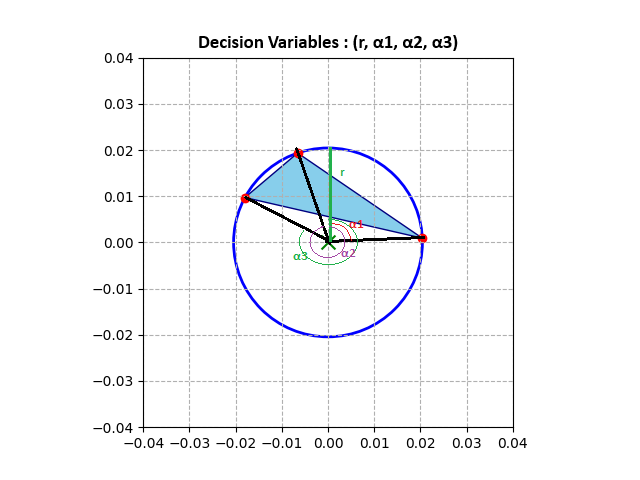
\includegraphics[width=0.8\textwidth]{fig/methodology/Polar Params.png}
    \caption{Polar parameterization of the suction-cup gripper.}
    \label{fig:polar_sc}
\end{figure}

Figure~\ref{fig:polar_sc} illustrates this parameterization. The common
radius \(r\) determines the radial distance of each cup center from the
gripper Tool Center Point (TCP), while the angles \(\alpha_i\) determine
the relative cup arrangement and its overall in-plane orientation.
For this thesis, the gripper height is fixed at \(z_0 = 0.326\)~m,
adopted from the suction-cup configuration employed in the bin-picking
demonstration conducted by Fraunhofer IPA. The Cartesian position of
cup \(i\) is obtained through the polar-to-Cartesian transformation
\begin{equation}
    \begin{aligned}
        \mathbf{p}_i &=
        \begin{bmatrix}
            r\cos(\alpha_i) \\
            r\sin(\alpha_i) \\
            z_0
        \end{bmatrix},
        \qquad \forall i\in\{1,2,3\}, \\
        &r,z_0\in\mathbb{R}, \qquad
        \alpha_i\in\mathbb{R},\quad
        \mathbf{p}_i\in\mathbb{R}^3,
        \qquad \forall i\in\{1,2,3\}.
    \end{aligned}
\end{equation}
The resulting Cartesian gripper configuration is
\begin{equation}
    \mathbf{P} = [\mathbf{p}_1,\mathbf{p}_2,\mathbf{p}_3],
    \qquad \mathbf{P}\in\mathbb{R}^{3\times 3}.
\end{equation}
Thus, optimization operates in the reduced four-dimensional parameter
space of \(\mathbf{q}\), while grasp evaluation operates on the derived
Cartesian configuration \(\mathbf{P}\).

All three angles are retained because grasp evaluation does not
separately explore rotations of the cup configuration about the local
\(z\)-axis, which is normal to the gripper plane. Changing all three
angles by the same amount rotates the configuration about the gripper
origin without altering the relative cup arrangement. Fixing
\(\alpha_1=0\) would instead constrain the first cup to the positive
direction of the grasp frame's first in-plane axis. Although the
remaining angles could describe different relative arrangements, their
overall orientation within that frame would be restricted. Retaining
all three angles therefore allows the optimizer to explore both cup
arrangement and in-plane orientation within the prescribed angular
bounds.

The common-circle constraint limits the search space while retaining
flexibility for diverse triangular cup arrangements. Separation
constraints prevent overlapping or degenerate layouts. A spatially
distributed triangular arrangement is adopted as a design assumption
to favour load distribution and resistance to external disturbances.
The triangle area serves as a geometric proxy for this distribution,
not as a guarantee of grasp stability, which also depends on seal
quality, available suction forces, workpiece properties, and external
loading.

\subsubsection{Parallel-Jaw Gripper and Contour Representation}
\label{subsubsec:two_finger_theory}

The parallel-jaw (PJ) gripper applies gripping forces through two opposing jaw
surfaces. Their contact contours determine how closely the gripper conforms
to the workpiece at the predefined grasp orientations. To represent smooth
contour variations with a compact design vector, the jaw contour is defined
by a cubic interpolating spline~\cite{Liu2024Topology,Hasan2024B-spline,Chapelier2022Spline-based}.

The contour lies in a plane spanned by the jaw depth and jaw length
directions. It is parameterized by the contour length $\ell_{\mathrm{gn}}$
and three depth offsets $h_1$, $h_2$, and $h_3$. These define five
interpolation points: the endpoints lie at zero depth, while the three
interior points are positioned at quarter intervals along the contour
length. The contour definition is
\begin{equation}
\mathbf{q}_{\mathrm{PJ}}
=
\begin{bmatrix}
\ell_{\mathrm{gn}} & h_1 & h_2 & h_3
\end{bmatrix}^{\mathsf{T}}
\in\mathbb{R}^4.
\end{equation}

The points on the cubic spline are defined as
\begin{equation}
\label{eq:jaw_contour_definition}
\begin{aligned}
\mathbf{s}_0&=(0,0),
\qquad \mathbf{s}_4=(0,\ell_{\mathrm{gn}}),
\\
\mathbf{s}_j&=
\left(h_j,\frac{j}{4}\ell_{\mathrm{gn}}\right)
\in\mathbb{R}^2,
\qquad \forall j\in\{1,2,3\}.
\end{aligned}
\end{equation}
The interpolation points lie on the resulting curve, unlike B-spline
control points. The endpoints at zero depth make the contour meet the
planar jaw face at both ends; the three interior offsets determine the
contour shape. Using four design variables provides a compact way to vary
the jaw profile while maintaining a smooth interpolating curve.

\begin{figure}[H]
    \centering
    \begin{minipage}[t]{0.48\linewidth}
        \centering
        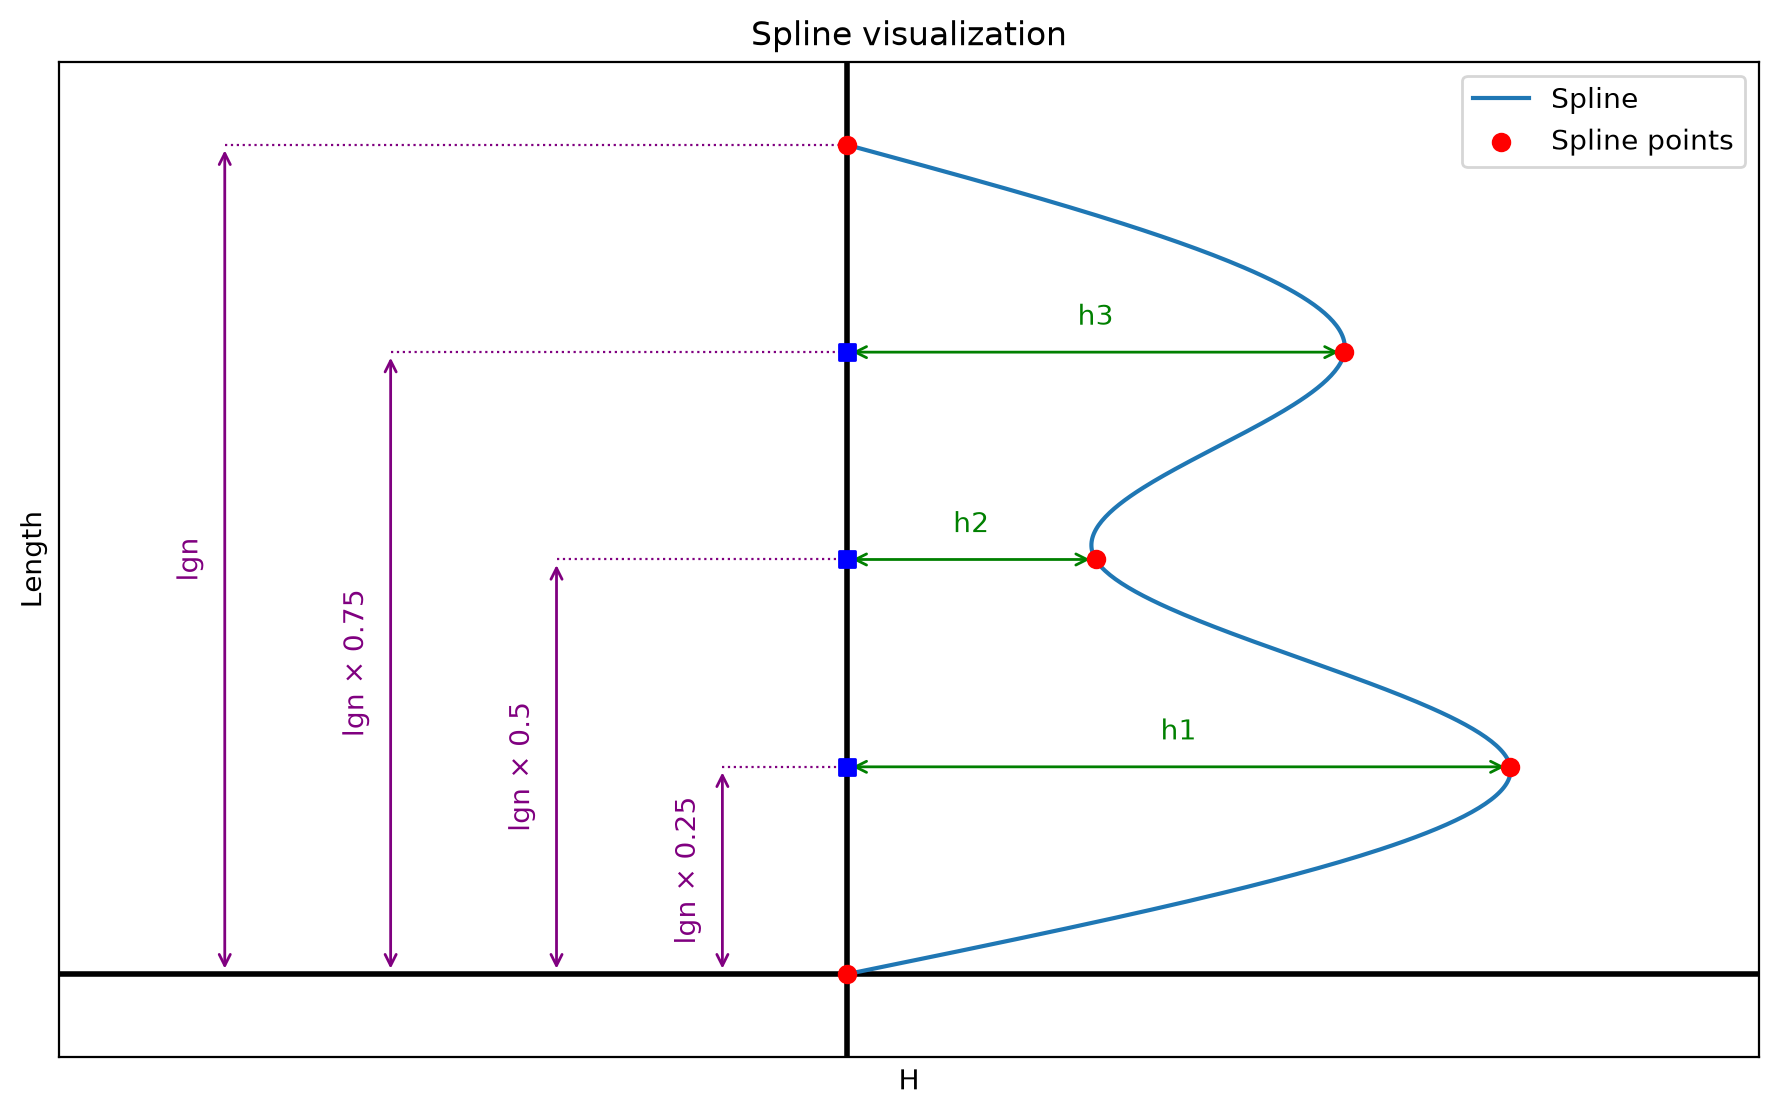
\includegraphics[width=\linewidth]{fig/methodology/spline.png}
        \par\smallskip
        (a)
    \end{minipage}\hfill
    \begin{minipage}[t]{0.48\linewidth}
        \centering
        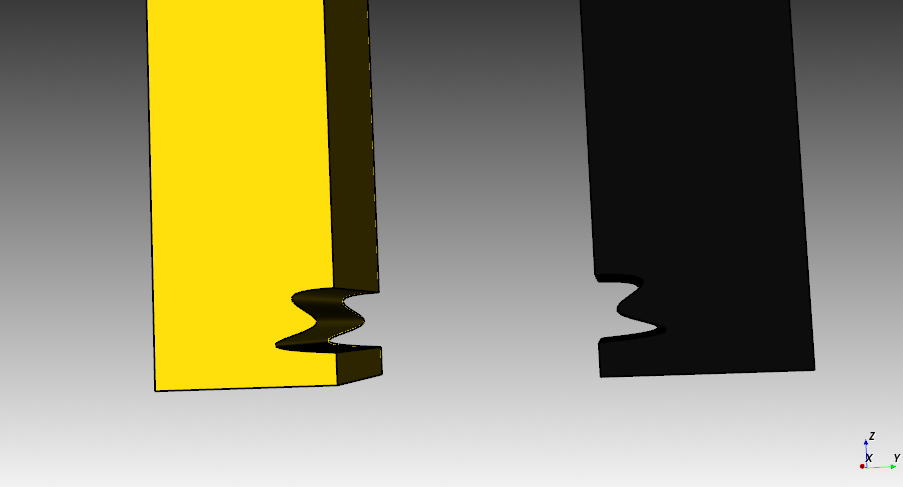
\includegraphics[width=\linewidth]{fig/methodology/PJGripper.png}
        \par\smallskip
        (b)
    \end{minipage}
    \caption{(a) Cubic spline interpolating the jaw-contour points.
    (b) Parallel-jaw gripper with the parameterized contours on its
    opposing jaw surfaces.}
    \label{fig:cubic_spline}
\end{figure}

Figure~\ref{fig:cubic_spline}(a) shows the interpolating spline, and
Figure~\ref{fig:cubic_spline}(b) shows the corresponding gripper geometry.
To construct the jaw, the contour is closed into a planar profile using
straight segments to a fixed cutting depth, then extruded through the jaw
depth to remove material from the basic jaw body. Geometry is generated
with CadQuery~\cite{cadquery2026} and exported in the mesh representation
used by the evaluation pipeline. Only $\ell_{\mathrm{gn}}$ and the three
offsets vary between candidates; all other jaw dimensions remain fixed.

Each candidate jaw geometry is generated once per evaluation request. For
each predefined workpiece orientation, the evaluator then voxelizes the
gripper and the rotated workpiece for the corresponding collision and
proximity calculations.


\subsection{Selection of Objective Functions for Multi-Suction Cup Gripper}
\label{subsec:methodology_objectives}

The objective functions define the properties used to distinguish effective gripper configurations. They must represent meaningful geometric
performance criteria while remaining computable through the available evaluation models~\cite{Todescato,Wolniakowski2017Task}.

For the multi-suction cup gripper, three objectives are used.

\subsubsection{Grasp diversity}
The first objective is the diversity of the valid grasps in position and orientation. A layout
that can grasp the workpiece in only one region is of limited use when the part arrives in varying
poses or when parts of its surface are blocked by fixtures or neighbouring objects. A diversity
measure captures this operational flexibility~\cite{Bo2023A,Pinskier2024Diversity-Based}.

\subsubsection{Number of distinct grasps}
Diversity alone does not show how many alternatives exist, because two well-separated grasps can
already produce a large spread. The number of distinct valid grasps is therefore the second
objective, as a measure of robustness: the more distinct grasps a layout offers, the more likely a
usable one remains when others are excluded by the scene or by reachability. Only distinct grasps
are counted, so that near-identical grasps cannot inflate the score.

\subsubsection{Support area}
The third objective is the area of the triangle spanned by the three cups. A wider support polygon
gives a longer lever arm against tilting moments, so the area serves as a stability proxy~\cite{madan2022realrobotchallenge2021}. It is a
purely geometric measure. The area objective itself does not model suction force, sealing quality,
material properties, or the centre of mass. The area was also chosen because it
conflicts with the first two objectives. A wide layout needs larger surface regions on which all
three cups can seal, which reduces both the number and the spread of feasible grasps. This conflict
is the central trade-off of the suction-cup design and is why a multi-objective formulation is
needed. All three objectives are normalized so that they remain comparable across workpieces and
within the hypervolume indicator.

\subsection{Selection of Objective Functions for Two-Finger Gripper}
\label{subsec:objective_two_finger_gripper}

For the two-finger gripper, the objectives measure the geometric
proximity between the workpiece and the two finger contours. This criterion
is evaluated for a fixed set of ten predefined workpiece orientations. The
method is inspired by Snuggle-Pack, which uses voxel-based collision and
proximity analysis to evaluate how closely an object fits its surroundings
~\cite{snuggle_pack}. Here, that general principle is adapted to
gripper evaluation where the workpiece is assessed relative to the two jaws, rather
than relative to objects and walls in a packing container.

\subsubsection{Geometric proximity score.}
For a given gripper design and workpiece orientation, the evaluator searches
for a relative placement of the workpiece between the jaws. Voxel
representations allow the evaluation to account for the three-dimensional
shape of both the workpiece and the finger contours. A proximity kernel gives
greater weight to workpiece voxels near each finger, so a higher score
indicates that the jaw geometry can be positioned close to the workpiece on
both sides. Collision checks exclude placements in which a jaw overlaps the
workpiece. The score is retained only when the resulting jaw opening satisfies
the implementation's feasibility condition; otherwise, the score for that
orientation is zero.

The proximity computation uses the FFT-based voxel analysis underlying
Snuggle-Pack. This is selected because it combines shape-aware, three-
dimensional evaluation with an efficient search over relative placements.
It therefore provides a practical way to compare many candidate spline
contours using the same geometric criterion, while accounting for collisions.
The method is used as a geometric conformity proxy; it does not directly
measure contact force, friction, material behaviour, or grasp stability.

\section{Optimization Library Selection}
\label{sec:methodology_library}

The evolutionary optimization algorithms are selected from the \texttt{pymoo} framework. \texttt{pymoo} provides a unified Python interface for
multi-objective evolutionary optimization, constraint handling, performance evaluation, and visualization. Using algorithms from a common framework
reduces implementation differences and improves the reproducibility of the comparison. The framework also provides established multi-objective
performance indicators, including hypervolume and inverted generational distance plus.~\cite{pymoo}

Bayesian multi-objective optimization is represented using the \texttt{Ax} platform and its underlying \texttt{BoTorch} functionality. Bayesian
optimization constructs probabilistic surrogate models of the black-box objective functions and uses an acquisition function to select promising
candidate evaluations. \texttt{Ax} provides the experiment-management interface, while \texttt{BoTorch} provides the probabilistic modeling and
acquisition-function capabilities.~\cite{olson2025ax,botorch}

The use of established open-source frameworks avoids the need to implement the optimization methods, surrogate models, and acquisition functions from
scratch. It also supports a more reproducible comparison between evolutionary and Bayesian optimization strategies.

\section{Algorithm Selection}
\label{sec:methodology_algorithm_selection}

For the experimental comparison, NSGA-II, NSGA-III, MOEA/D, SMS-EMOA, CMOPSO, and multi-objective Bayesian optimization are selected.

The selection was made to compare different approaches to multi-objective search under the same gripper-design problems and evaluation budget.
Including algorithms with different search principles reduces the extent to which the comparison is limited to variations of a single optimization
strategy. It also allows the experiments to determine whether the relative performance depends on the selected gripper type or workpiece.

\begin{itemize}
    \item \textbf{NSGA-II} is selected as the baseline algorithm for the population-based comparison.

    \item \textbf{NSGA-III} is included to compare the NSGA-II baseline with an alternative that organizes the search using predefined reference
    directions.

    \item \textbf{MOEA/D} is selected to include a decomposition-based approach and to examine how this formulation performs on the objective
    trade-offs of the gripper-design problems.

    \item \textbf{SMS-EMOA} is included as an indicator-based approach. Its selection also permits investigation of an algorithm whose search is
    directly associated with hypervolume, one of the performance indicators used in this thesis.

    \item \textbf{CMOPSO} is selected to include a swarm-based search method and thereby extend the population-based comparison beyond evolutionary
    algorithms.

    \item \textbf{Multi-objective Bayesian optimization} is included as a model-based alternative to the population-based methods. This allows its
    performance under a limited evaluation budget to be compared with that of the other selected algorithms.
\end{itemize}

Together, these algorithms form a deliberately varied comparison set containing dominance-based, reference-direction-based, decomposition-based,
indicator-based, swarm-based, and model-based approaches. The experiments use this selection to determine which approaches provide suitable
convergence, trade-off representation, and consistency for the suction-cup and parallel-jaw gripper-design problems.
\section{Workpiece Selection}
\label{sec:methodology_workpiece_selection}

Four geometrically diverse workpieces are selected to examine whether
optimization behaviour changes across planar, cylindrical, elongated,
and free-form geometries. Such diversity is relevant because algorithm
performance can depend on the feasible design space and optimization
landscape~\cite{Cenikj2022SELECTOR:,Yazdani2020Benchmarking}.

\begin{figure}[htbp]
    \centering
    \begin{subfigure}[t]{0.47\textwidth}
        \centering
        
\includegraphics[
            width=\linewidth,
            height=0.17\textheight,
            keepaspectratio
        ]{fig/methodology/IPAIntermediatePlate.png}
        \caption{IPA Intermediate Plate}
        \label{fig:workpieces_IPAIntermediatePlate}
    \end{subfigure}\hfill
    \begin{subfigure}[t]{0.47\textwidth}
        \centering
        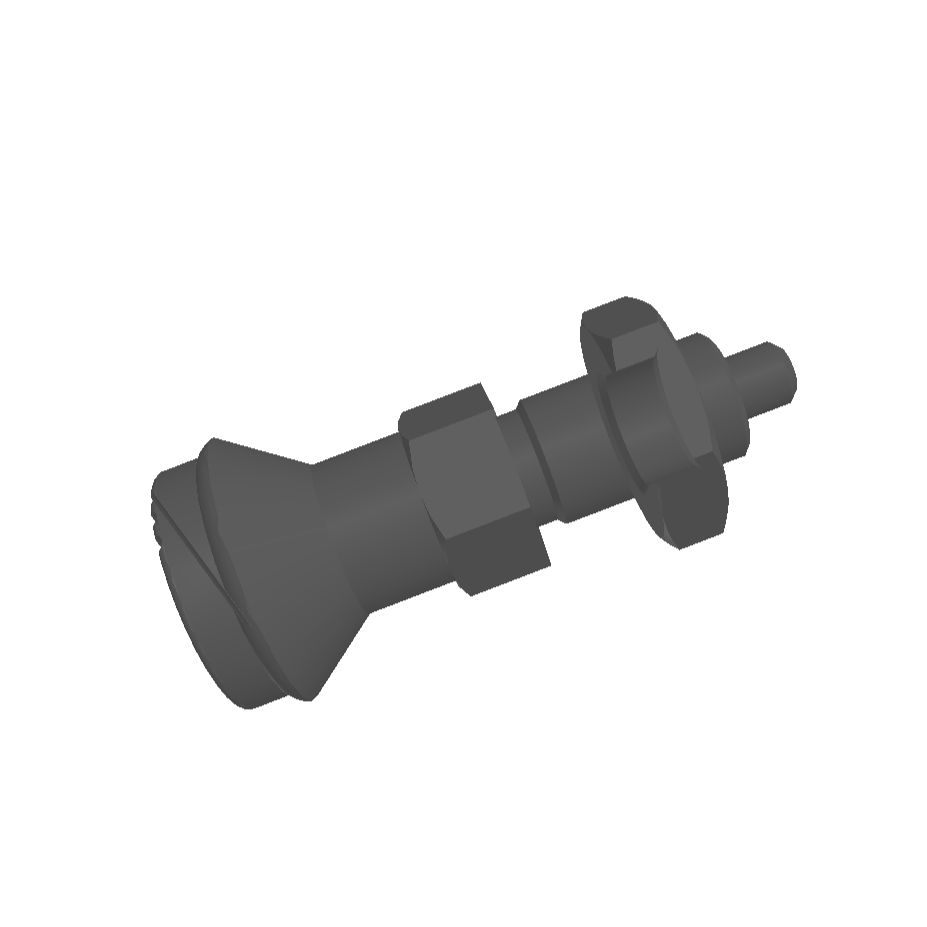
\includegraphics[
            width=\linewidth,
            height=0.17\textheight,
            keepaspectratio
        ]{fig/methodology/knob.png}
        \caption{Knob}
        \label{fig:workpieces_Knob}
    \end{subfigure}

    \par\medskip

    \begin{subfigure}[t]{0.47\textwidth}
        \centering
        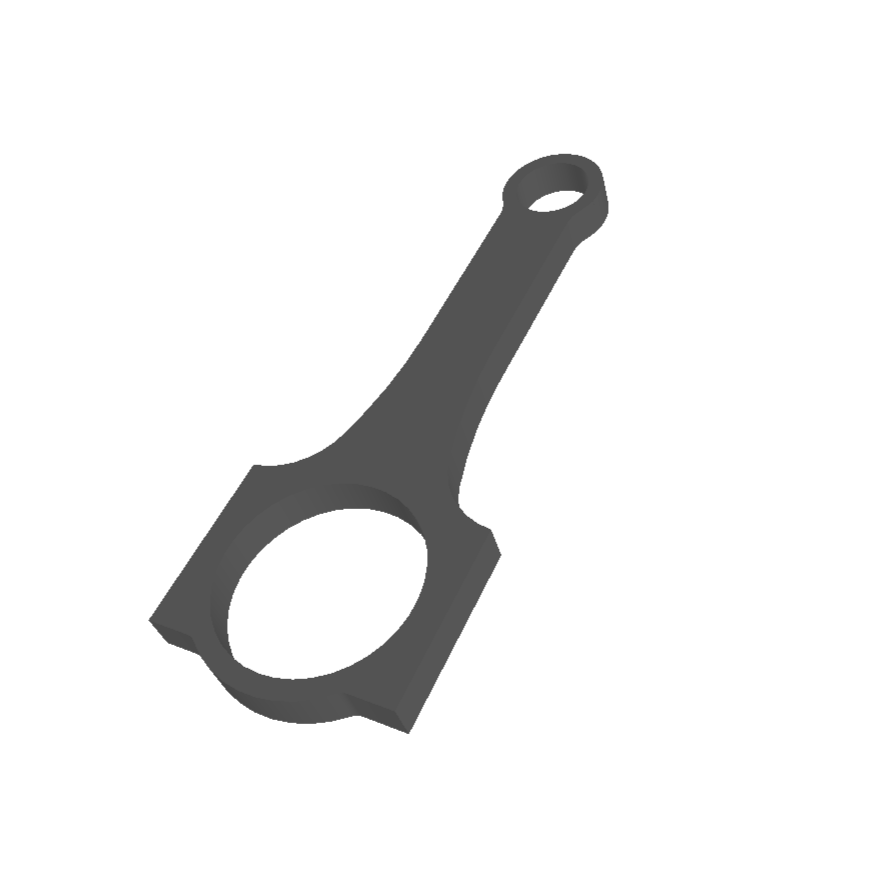
\includegraphics[
            width=\linewidth,
            height=0.17\textheight,
            keepaspectratio
        ]{fig/methodology/connecting_rod.png}
        \caption{Connecting rod}
        \label{fig:workpieces_ConnectingRod}
    \end{subfigure}\hfill
    \begin{subfigure}[t]{0.47\textwidth}
        \centering
        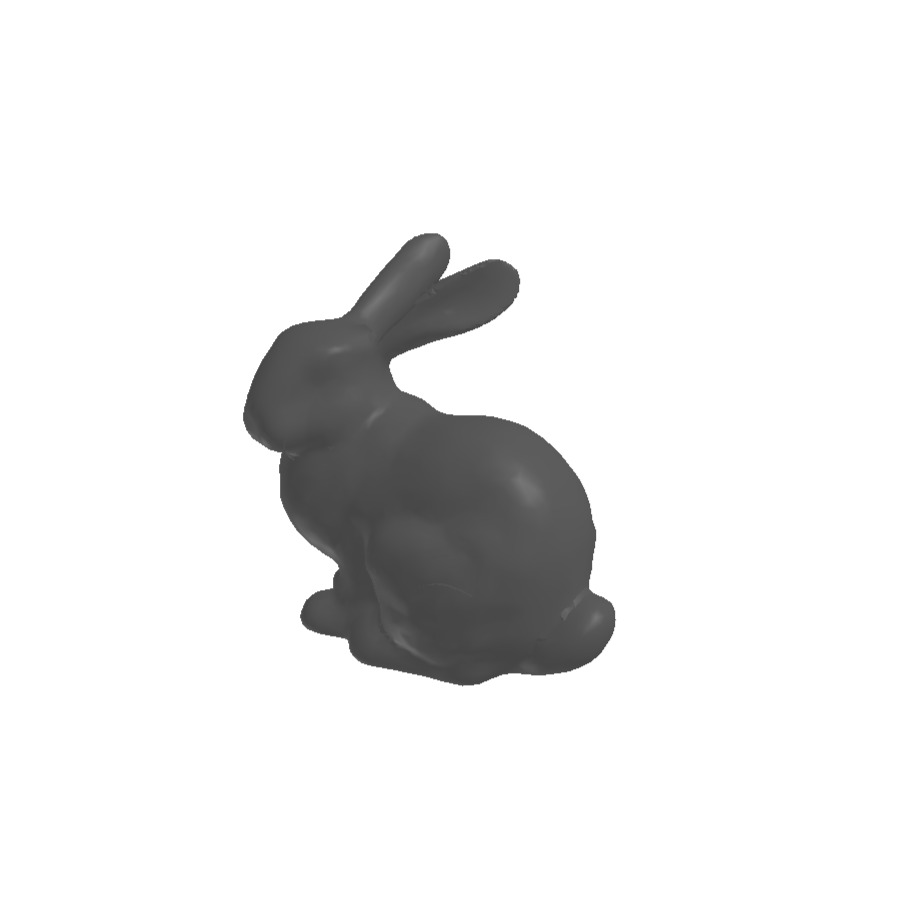
\includegraphics[
            width=\linewidth,
            height=0.17\textheight,
            keepaspectratio
        ]{fig/methodology/Bunny.png}
        \caption{Stanford Bunny}
        \label{fig:workpieces_Bunny}
    \end{subfigure}

    \caption{Selected workpieces representing planar, cylindrical,
    elongated, and free-form geometries.}
    \label{fig:workpieces}
\end{figure}

The \textbf{IPAIntermediatePlate}
(Figure~\ref{fig:workpieces}(\subref{fig:workpieces_IPAIntermediatePlate}))
is a regular industrial component with large planar regions and straight
edges, representing structured, prismatic workpieces.
The \textbf{Knob}
(Figure~\ref{fig:workpieces}(\subref{fig:workpieces_Knob}))
is predominantly cylindrical and rotationally symmetric, with a stepped
circumferential profile.
The \textbf{ConnectingRod}
(Figure~\ref{fig:workpieces}(\subref{fig:workpieces_ConnectingRod}))
is a flat, elongated component with a high length-to-width ratio and two
circular ends connected by a narrow shaft, representing slender,
asymmetric geometries.
The \textbf{Stanford Bunny}
(Figure~\ref{fig:workpieces}(\subref{fig:workpieces_Bunny}))
provides a free-form, non-symmetric geometry with curved surfaces,
irregular features, and substantial local variation.

Each workpiece defines an independent optimization instance, as described
in Section~\ref{subsec:study_structure}.

\section{Comparative Experimental Design}
\label{sec:methodology_comparative_experiments}

A controlled comparative design is adopted to reduce differences unrelated
to the optimization methods. For a given gripper--workpiece instance,
all algorithms use the same geometric parameterization, objective
functions, variable bounds, feasibility conditions, and evaluation service.
Evaluation budgets are matched within optimizer families. Comparisons
between evolutionary and Bayesian optimization therefore account for
evaluation count and wall-clock time.

Because the selected optimization methods contain stochastic components, independent repetitions are used to examine performance variability and
robustness. Comparisons are performed within the same problem instance. Results from different workpieces or gripper
types are not combined into one optimization problem or one Pareto front.

\section{Performance Indicators}
\label{sec:methodology_performance_indicators}

Algorithm performance is evaluated using three indicators: inverted
generational distance plus (IGD+), hypervolume, and total optimization
runtime. Together, they characterize approximation-set quality and
computational cost.

IGD+ is selected to assess how well an optimization run approximates the best trade-offs identified for a given gripper--workpiece problem. It is
useful in this thesis because it considers both proximity to the reference front and the representation of different regions of that front. This
enables the algorithms to be compared based on the overall quality of their approximation sets rather than on individual objective values alone.

Hypervolume is selected as an aggregate measure of approximation-set quality. It provides a single value that reflects both convergence and
the extent of the represented objective-space trade-offs. Considering the final value attained during a run is particularly relevant for the
investigated black-box optimization problems because it identifies the best approximation quality reached within the available optimization budget,
even when the quality of the population varies during a run.

Total optimization runtime measures the computational cost of a complete
run, including candidate generation, objective evaluation, and optimizer
updates. It complements the quality indicators by showing the time
required to obtain the resulting approximation set. Runtime comparisons
are interpreted alongside the evaluation budgets, which differ between
evolutionary and Bayesian optimization.

The three indicators therefore provide complementary assessments of
approximation quality and computational effort. Their values across
independent repetitions are used to characterize both performance and
its variability.


\nomenclature{$\mathbf{q}_{\mathrm{SC}}$}{Four-dimensional decision vector defining the suction-cup gripper configuration}
\nomenclature{$\mathbf{q}_{\mathrm{PJ}}$}{Four-dimensional decision vector defining the parallel-jaw gripper contour}